\chapter{Desarrollo}\label{sec:capitulo3}
\thispagestyle{empty}

\begingroup
\rightskip0.5cm
\small

\endgroup

\section{Estableciendo parámetros a medir}%-------------------------------------
  \par Como ya se mencionaron antes los estandares internacionales establecen:
  \begin{itemize}
   \item Valores nominales de la red eléctrica
   \item Espcificaciones de los medidores inteligentes
         \begin{itemize}
          \item Eléctricas
          \item Medición (BUSCAR OTRO TERMINO)
         \end{itemize}
  \end{itemize}

  \subsection{Eléctricas}
  \par La norma EDC E-354-1608 establece los valores nominales de la red eléctrica,
  los cuales deben ser medidos por el medidor inteligente.

  \begin{table}[H]
   \centering
   \caption{\label{Valores_nominales_re}Valores nominales de operacion de la red eléctrica, extracto norma E-354-D-1608}
   \resizebox{\textwidth}{!}{
    \begin{tabular}{cccc}
     \hline
     \textbf{\begin{tabular}[c]{@{}c@{}}Característica\\ Medidor\end{tabular}} & \multicolumn{3}{c}{\textbf{Medición Eléctrica}}                                                         \\ \hline
     Tipo                               & 1F, 2 Hilos                                     & 1F, 3 Hilos               & 3F, 4 Hilos               \\
     Rango de intensidad (A)            & 10-60                                           & 15-80                     & 15-100                    \\
     Tensión nominal (V)                & 120                                             & \begin{tabular}[c]{@{}c@{}}2 x 120/240\\ 2 x 240/480\end{tabular} & \begin{tabular}[c]{@{}c@{}}3 x 208Y/120\\ 3 x 240/2 x 120\\ 3 x 416Y/240\\ 3 x 480Y/277\end{tabular} \\
     Rigidez dielectrica?? (KV)         & 4                                               & 4                         & 4                         \\
     Frecuencia (Hz)                    & 60                                              & 60                        & 60                        \\ \hline
    \end{tabular}}
  \end{table}

  \par La tabla \ref{Valores_nominales_re} es un estracto de la norma ya mencionada en
  de la cual determinamos los valores en el cual operan los medidores inteligentes;
  frecuencia de 60 Hz, 120 V nominales y corriente entre 10-60 A.

  \subsection{Medición}

  La norma IEC 61000-4-30 especifica que los medidores de clase B deben ser capaces
  de medir hasta el 30avo armónico.

  \textbf{NORMA QUE ESTABLECE LOS ERRORES PORCENTUALES PERMITIDOS}

\section{Tarjeta de acondicionamiento}%-----------------------------------------


\section{Eleccion de dispositivo para procesamiento}%----------------------------
  \par Se evaluaron unidades de procesamiento de distintas compañias y los
  disponibles en el laboratorio del grupo de Sistemas Industriales y Electrónica
  de Potencia capaces de realizar las funciones del MEI. Por parte de la empresa
  Texas Instruments los dispositivos TMS320F28027 y TMS320F28069 pertenecientes
  a la familia C2000 - Piccolo, de la empresa National Instruments el myRIO-1900
  y por último de la familia Intel el Arduino UNO.

  Las caracteristicas evaluadas de cada microcontrolador son las siguientes:
  \begin{itemize}
   \item Velocidad de adquisición
   \item Resolución de ADC
   \item Velocidad de procesamiento
   \item Conectividad
   \item Acceso directo a memoria
  \end{itemize}

  \begin{table}[H]
   \centering
   \caption{\label{Especificaciones_dispositivos_comerciales_evaluados}Especificaciones de los dispositivos comerciales evaluados}
   \resizebox{\textwidth}{!}{\begin{tabular}{ccccc}
     \hline
     \textbf{Dispositivo}      & \textbf{Arduino Uno} & \textbf{myRIO-1900} & \textbf{TMS320F28027} & \textbf{TMS320F28069} \\ \hline
     \begin{tabular}[c]{@{}c@{}}Frecuencia de \\ muestreo\end{tabular} & 8950 Hz              & 40 KHz              & 3.4 MHz               & 4.6 MHz               \\
     \begin{tabular}[c]{@{}c@{}}Velocidad de\\ procesamiento\end{tabular} & 16 MHz               & 667 MHz             & 60 MHz                & 90 MHz                \\
     Conectividad              & Serial               & Serial / Wifi       & Serial                & Serial                \\
     \begin{tabular}[c]{@{}c@{}}Acceso directo \\ a memoria\end{tabular} & No                   & Si                  & Si                    & Si                    \\ \hline
    \end{tabular}}
  \end{table}

  \subsection{Frecuencia de muestreo (MODIFICAR ARMONICO)}
  \par Los estandares internaciones (averiguar que estandar) de la IEC establecen
  que los medidores inteligentes de clase B, los utilizados en las zonas residenciales,
  deben detectar al menos hasta el 51avo armónico. La frecuencia de la señal a medir es de 60 Hz, la
  correspondiente a la red eléctrica en Venezuela, ubicando el 51avo armónico a una frecuencia de
  3060 Hz. Según el teorema de Nyquist se requiere una frecuencia de muestreo de al menos el doble
  de dicha frecuencia, 6080 Hz.
  \par Los ADC de todos los dispositivos se encuentran multiplexados, lo que implica que
  la frecuencia de muestreo se dividira por el numero de señales a obtener. En este caso
  se utilizaran dos canales, en uno se obtendra la señal de voltaje y en el otro la de
  corriente. Duplicando asi la frecuencia de muestreo necesaria para muestrear la señal,
  12.16 KHz.

  \subsection{Velocidad de procesamiento y acceso directo a memoria}
  \par Al ser un sistema embebido y en tiempo real, es necesario que el dispositivo
  sea capaz de realizar grandes cantidades de instrucciones y ejecuciones en paralelo.
  Por otro lado los dispositivos que posea acceso directo a memoria son mas capaces de
  realizar operaciones debido a que este acceso es capaz de trabajar en paralelo con
  el procesamiento de los datos (ARREGLAR).

  \subsection{Comunicación}
  \par Siguiendo los estandares (averiguar estandar) para la comunicacion de los
  medidores inteligentes, se recomienda que el dispostivo sea capaz de conectarse a una
  red y enviar datos mediante el protocolo TCP/IP. \\

  \par Teniendo en cuenta todo esto tomamos como parametro mas importante la frecuencia de
  muestreo, descartando de este modo al dispositivo Arduino Uno que solo posee una
  máxima frecuencia de 8950 Hz con un canal. Los dispositivos restantes cumplen con
  sosobra la frecuencia de muestreo minima necesaria, teniendo que tomar en cuenta los
  siguientes aspectos. La velocidad de proceseamiento en los tres dispositivos es
  sumamente elevada y ademas de esto cuentan con la capacidad de acceso directo a
  memoria dando un uso mas optimizado de sus recursos. Sin embargo por la parte de
  comunicacion los dispositivos de Texas Instruments requieren de modulos extras
  para obtener conexión WIFI y poder transmitir los datos por el protocolo TCP/IP,
  dejando asi en ventaja al dispositivo myRIO. De tal modo se eligio el dispositivo
  myRIO ya que cumple con todas las caracteristicas necesarias y este ya se encuentra
  disponible en los laboratorios de la agrupación al contrario de los TI que es necesario
  realizar su compra.

\section{Programación}
  \par En la sección anterior se describio el proceso de acondicionamiento de la señal, de tal modo que la señal a digitalizar se encuentre en el rango de entrada del ADC del dispositivo myRIO. Al poseer la señal digitalizada se procede a realizar el procesamiento de los datos para obtener los parametros electricos deseados.

  \par (EXPLICAR COMO SE PUEDE PROGRAMAR EL FPGA Y EL MYRIO) El dispositivo myRIO se programa mediante el software de desarrollo grafico Labview. Para llevar acabo el procesamiento de datos se establecieron modulos con funciones especificas con el fin de realizar una programación mas ordenada y eficiente. Estos modulos son:

  \begin{itemize}
    \item FPGA
    \item myRIO - Sistema Operativo
    \item PC - Host
  \end{itemize}
  \begin{figure}[H]
    \centering
    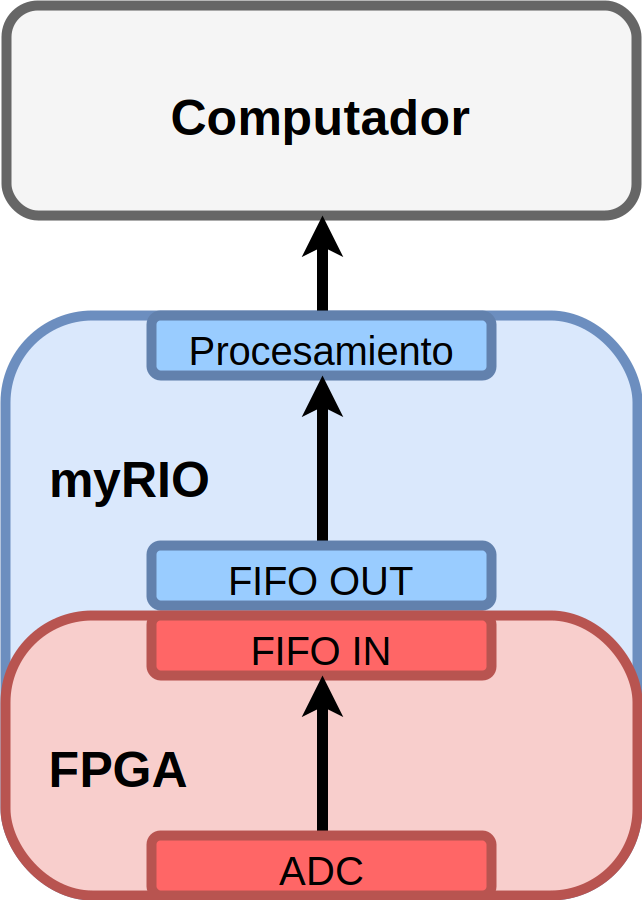
\includegraphics[width=0.4\textwidth]{../Imagenes/estructura_procesamiento.png}
    \caption{Hardware utilizado para el procesamiento (AGREGAR HOST)}
    \label{fig:Hardware_Pro}
  \end{figure}s

  \subsection{FPGA}
    \par En este modulo se define la frecuencia de muestreo a utilizar. Se desea detectar el armónico 50 de la señal de 60Hz, por lo tanto la frecuencia de muestreo mínima a utilizar según el teorema de Nyquist sera de 6KHz, agregando a esto la utilización de un ADC multiplexado es necesario duplicar esta frecuencia para lograr obtener la medición de dos canales, voltaje y corriente. Por lo tanto estableceremos como mínimo una frecuencia de 12KHz, implicando asi que la cantida de muestras pertinentes a un periodo de la señal a obtener seran de 200 muestras.

    \par El algoritmo de adquisición de los datos es el siguiente:
    \begin{figure}[H]
        \centering
        \includegraphics[width=0.4\textwidth]{../Imagenes/Algoritmo_FPGA.png}
        \caption{Algoritmo FPGA}
        \label{fig:Algo_FPGA}
    \end{figure}

    \par El programa estara estructurada por una estructura while loop y un flat sequence. Esta última establecerá primeramente el tiempo de muestreo, el cual es el inverso a la frecuencia de muestro mencionada anteriormente, 83.34us, sin embargo el tiempo de muestreo en el modulo debe ser un numero entero por lo cual se redondea este a 83us. En la siguiente secuencia se adquiriran los datos del puerto ADC y se almacenaran en la memoria directa de estructura tipo FIFO. En la figura \ref{fig:DB_FPGA} se encuentra el diagrama de bloques del programa, este no cuenta con un panel frontal debido a que no es necesario establecer o visualizar valores en este modulo.

    \begin{figure}[H]
        \centering
        \includegraphics[width=0.4\textwidth]{programa_FPGA.png}
        \caption{Diagrama de bloques del FPGA}
        \label{fig:DB_FPGA}
    \end{figure}

  \subsection{myRIO}
    \par En este modulo se llevara acabo el procesamiento de los datos el cual involucra el cálculo de los parámetros, almacenamiento y la comunicacion con el dispositivo recolector, creando un VI respectivo para cada tarea.
    \subsubsection{Procesamiento}
      \par Lo primero a realizar en este VI es la inicializacion de los elementos a utilizar: modulo FPGA, Buffer de salida de la memoria directa, constantes. Lo siguiente a esto es un algoritmo que pose como estructura productor-consumidor.
      \subsubsubsection*{Productor}
        \par En esta sección se extraera de la memoria de acceso directo y se depositara en una cola, la cantidad de muestras respectivas a 6 periodos, 1200 muestras, de tal modo que esta no exceda su capacidad de almacenamiento.

        \par El tipo de datos extraido de la memoria se encontrara en forma vectorial, en la figura (REFERENCIA) se logra observar esta.
        \begin{figure}[H]
            \centering
            \includegraphics[width=0.4\textwidth]{../Imagenes/estructura_datos.png}
            \caption{Estructura de datos}
            \label{fig:Est_dat}
        \end{figure}

      \subsubsubsection*{Consumidor}
        \par Como es conocido por el algoritmo el consumidor debera extraer datos para su utilización, según el estandar (REFERENCIA) la cantidad de datos respectivos a 12 periodos es necesaria para realizar el procesamiento apropiadao de la data. Los datos extraidos se concatenaran para obtener un vector con las dimensiones 2x1200.

        \par Aqui se realizará el cálculo de los parametros electricos y su almacenamiento

      \subsubsubsection{Calculo de parametros}


    \subsubsection{Almacenamiento}
    \subsubsection{Comunicación}
  \subsection{Host}
    \subsubsection{Comunicación}
    \subsubsection{Interfaz}
